\begin{document}

\subsection{Опишите основные уравнения для моделирования фильтрации потока.}

\includegraphics[width=\textwidth, page=7]{1_Производительность_скважин_на_отправку.pdf}

Закон Дарси -- основной закон фильтрации жидкостей и газов в пористой среде.
\\

Откуда появляются другие виды закона фильтрации?

На самом деле теоретически можем вывести закон фильтрации как разложение тензора диссипативных напряжений.
И дальше брать необходимое количество слагаемых в этом разложении.
\\

При больших скоростях зависимость между градиентом давления и скоростью фильтрации нелинейна (хорошее совпадение с экспериментальными данными даёт квадратичная зависимость -- закон фильтрации Форхгеймера).
\\

Выражение для фильтрации с начальным градиентом давления задаёт порог давления, ниже которого жидкость не течёт.
В основном используется для существенно вязкопластичных жидкостей (например, битумов).
\\

Из закона Дарси, уравнения неразрывности и соотношения на сжимаемость флюида можем получить основное уравнение для моделирования фильтрации потока (уравнение пьезопроводности).

\begin{figure}[H]
\textbf{Уравнение пьезопроводности}

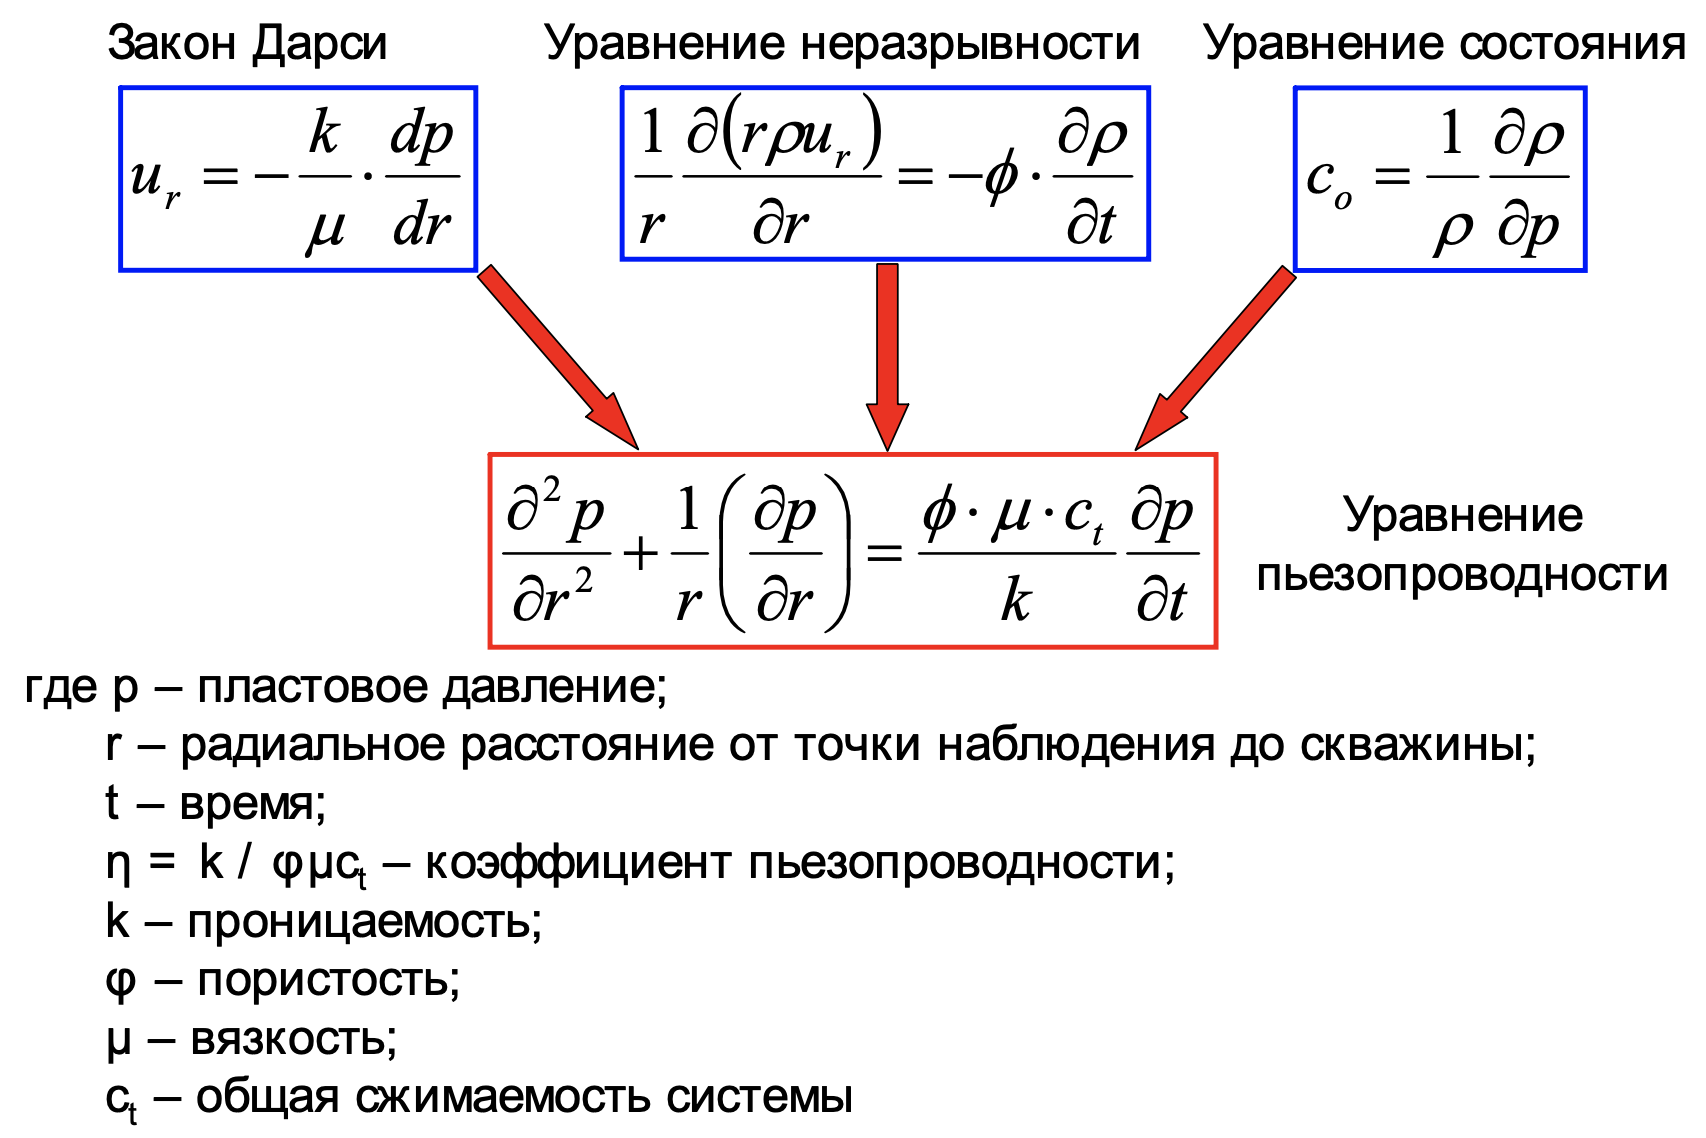
\includegraphics[width=\textwidth]{get_piezoconductivity}
\end{figure}

Уравнение пьезопроводности -- основное уравнение для моделирования фильтрации потока.
\\

Коэффициент пьезопроводности пласта -- коэффициент, характеризующий темпы распределения пластового давления в условиях упругого режима, равный отношению коэффициента проницаемости пласта к произведению вязкости жидкости и её сжимаемости.

\end{document}